% !TEX root =  ../main_manuscript.tex 
\section{Introduction}
\label{sec:introduction}
Chronic non-communicable diseases (e.g., cancer, lung, cardiovascular diseases) cause 60--70\% of human deaths worldwide~\citep{world2014global}. Often patients diagnosed with an early-stage disease undergo repeated surveillance \textit{tests} to timely detect disease \textit{progression}, a non-terminal event. Gold standard surveillance tests utilized for this purpose are usually invasive. For example, in prostate cancer surveillance, progression from low to high-grade is detected using biopsies~\citep{bokhorst2015compliance}. Similarly, endoscopies are employed in Barrett's esophagus~\citep{streitz1993endoscopic}, colonoscopies for colorectal cancer~\citep{krist2007timing}, and bronchoscopies for detecting lung transplant~\citep{mcwilliams2008surveillance} deterioration.

Often fixed schedules (e.g., biannually) are utilized for invasive tests in surveillance~\citep{mcwilliams2008surveillance,bokhorst2015compliance,krist2007timing}. Since tests are conducted periodically, there is always a time delay in detecting progression (Figure~\ref{fig:delay_explanation}). The frequency/timing of tests and the corresponding time delay in detecting progression, manifest the burden and benefit of test schedules, respectively. Tests are burdensome because they may cause pain and/or severe medical complications~\citep{loeb2013systematic,krist2007timing}, and consequently patients may not always comply with frequent tests~\citep{bokhorst2015compliance}. On the other hand, detecting progression timely can provide a larger window of opportunity for curative treatment. In this regard, one-size-fits-all fixed schedules impose an equal but unnecessary burden on all patients, because many early-stage patients can be slow/non-progressing.

\begin{figure}
\centerline{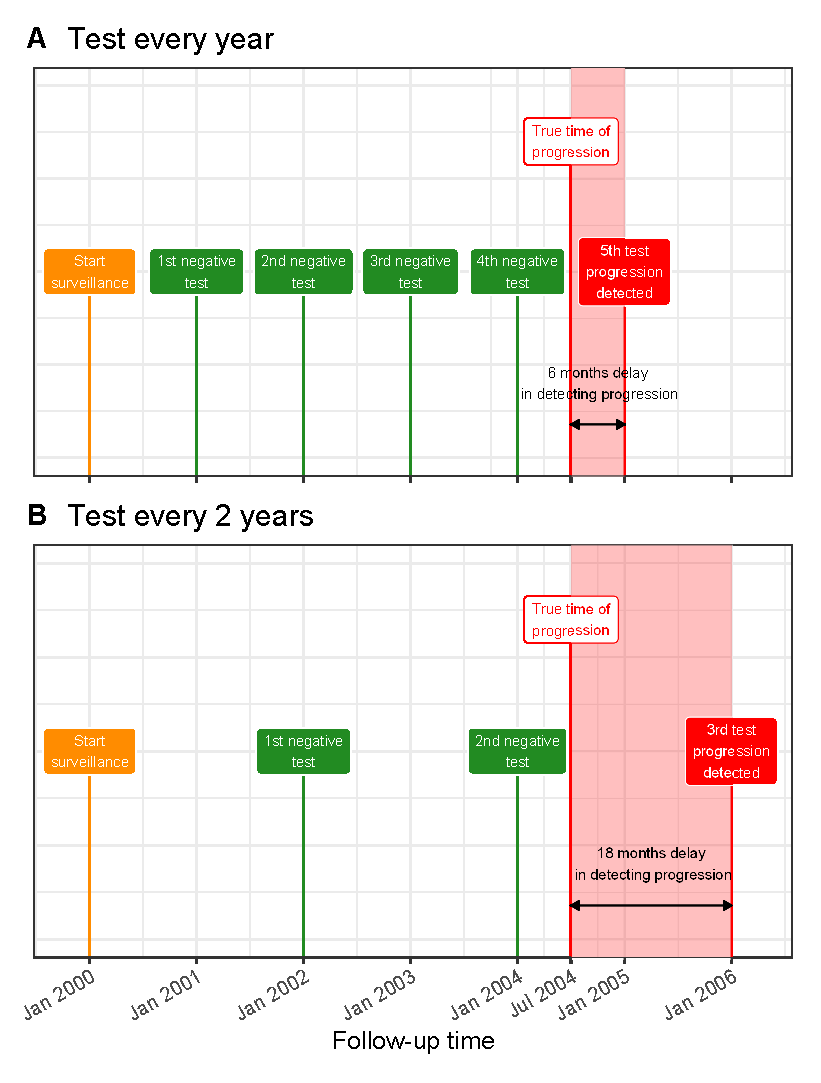
\includegraphics{images/delay_explanation.eps}}
\caption{\textbf{Trade-off between the number of invasive tests and time delay in detecting progression (non-terminal event of interest):} The true time of progression for this patient July 2004. More frequent invasive tests in \textbf{Panel~A} lead to a shorter time delay in detecting progression than less frequent invasive tests in \textbf{Panel~B}. Since invasive tests are conducted periodically, the time of progression is observed as an interval. For example, between Jan~2004--Jan~2005 in \textbf{Panel~A} and between Jan~2004--Jan~2006 in \textbf{Panel~B}.} 
\label{fig:delay_explanation}
\end{figure}

In this work, we aim to balance the number of invasive tests and the time delay in detecting progression better than fixed schedules. Specifically, we intend to create personalized schedules that utilize patient-specific clinical data accumulated over follow-up. In surveillance, this data includes baseline characteristics; previous invasive test results; and auxiliary longitudinal outcomes such as biomarkers, physical examination, and medical imaging measurements, etc. Previous attempts at personalized scheduling can be divided into three categories. First, heuristic approaches such as decision making flowcharts, e.g.,~\citet{bokhorst2015compliance}. However, flowcharts discretize continuous clinical outcomes, often exploit only the last measurement, and ignore the measurement error in observed data. Second, partially observable Markov decision processes~\citep{alagoz2010operations, steimle2017markov} for personalizing test decisions. Although, the curse of dimensionality limits their application with continuous longitudinal outcomes. Third, personalized schedules obtained by optimizing an explicit utility function of the clinical parameters of interest~\citep{bebu2017optimal,rizopoulos2015personalized}, \textcolor{Green}{including our previous works on scheduling biopsies in prostate cancer~\citep{tomer2019personalized,tomer2020webapp}}. In this work, we will employ the third approach.

In our methodology, we first develop a full specification of the joint distribution of the patient-specific longitudinal outcomes and the time of \textit{progression}. To this end, we employ joint models for time-to-event and longitudinal data~\citep{tsiatis2004joint,rizopoulos2012joint} because they are also inherently personalized. Specifically, they exploit patient-specific random effects~\citep{mcculloch2005generalized} to model longitudinal outcomes without discretizing them. Subsequently, we input the accumulated clinical data of a new patient into the fitted model, to obtain their patient-specific cumulative-risk of progression at their current and future follow-up visits. We then create personalized schedules by planning tests on future visits where the predicted conditional cumulative-risk is above a particular \textit{threshold} (e.g., 5\% risk). We automate the choice of this threshold and the resulting schedule. Specifically, we optimize a utility function of the expected number of tests (burden) and time delay in detecting progression (shorter is beneficial) for different risk threshold based personalized schedules. We estimate these two quantities in a patient-specific manner for following any schedule, by utilizing the predicted risk profile of the patient. Patients/doctors can employ these quantities to objectively compare various personalized and fixed schedules.

We are motivated by the problem of scheduling biopsies~\citep{nieboer2018active} in the world's largest prostate cancer active surveillance study PRIAS~\citep{bokhorst2015compliance}. \textcolor{Green}{It has 7813 patients (1134 cancer progressions) with 104904 longitudinal measurements~\citep{tomer2020webapp}}. At inclusion, patients have low/very-low grade cancer, often over-diagnosed due to prostate-specific antigen (PSA) based screening~\citep{crawford2003epidemiology}. Active surveillance aims to delay serious treatments (e.g., surgery, chemotherapy) until cancer progression is detected. To this end, patients are monitored continually via serum PSA (ng/mL), digital rectal examination (DRE) for shape/size of the tumor, and biopsy Gleason grade group~\citep{epsteinGG2014}. Among these, the strongest indicator of cancer-related outcomes is the Gleason grade group. Hence, when it increases (cancer progression) treatment is commonly advised. In this regard, most often biopsies are scheduled annually~\citep{loeb2014heterogeneity}. Although, annual schedule leads to many unnecessary biopsies in slow/non-progressing patients (50\% proportion in PRIAS). Biopsy burden and patient non-compliance to frequent biopsies~\citep{bokhorst2015compliance} has raised concerns regarding the optimal biopsy schedule. Since prostate cancer has the second-highest incidence among all cancers in males~\citep{GlobalCancerStats2012}, individualized biopsy schedules can reduce the burden of biopsies numerous patients worldwide.

The rest of the paper is as follows. Section~\ref{sec:jointmodel} briefly introduces the joint modeling framework. In Section~\ref{sec:schedule}, we present the methodology for personalized schedules and then demonstrate them for biopsies in real PRIAS patients in Section~\ref{sec:results}. Lastly, in Section~\ref{sec:sim_study}, we show the efficacy of personalized schedules via a realistic simulation study based on PRIAS patients.